\documentclass[11pt]{article}

% Math
\usepackage{amsmath, amssymb, amsfonts, mathtools}

% Page layout
\usepackage[margin=1in]{geometry}

% Optional useful packages
\usepackage{physics}      % \bra, \ket, \dv, \pdv, etc.
\usepackage{bm}           % bold math symbols
\usepackage{bbm}
\usepackage{enumitem}     % better lists
\usepackage{graphicx}     % Required for inserting images
\usepackage{subcaption}   % Required for the subfigure environment
\usepackage{hyperref}     % links
\hypersetup{
    colorlinks=true,       % false: boxed links; true: colored links
    linkcolor=blue,        % color of internal links (sections, pages, etc.)
    citecolor=green,       % color of citation links to bibliography
    % filecolor=magenta,     % color of file links
    urlcolor=blue,         % color of external website links
    % allcolors=blue       % uncomment this if you want ALL links to use one color
}

\title{Weekly Update}
\author{Reza Asakereh}
\date{Last Update: \today}

\begin{document}

\maketitle

\section{Main Findings}
\subsection{DB-Sorter}
\textbf{quick background.} DB-sorter uses the sorting characteristic of DB flow to find ground state or excited states of a hamiltonian $H$ using a diagonal matrix $D$ that has an engineered order in its diagonal elements (usually increasing). We compare three different diagonals in terms of spectral gaps and synthesis complexity. 
\\

\textbf{Findings:}
\begin{itemize}
    \item I simulated the method for three other hamiltonian models: TFIM, XXZ, and J1/J2 model. I tried three different diagonal choices for $D$. Cool down happens in all. See \href{https://github.com/rasakereh/double-bracket-algo/blob/master/examples/different_diagonals.py}{GitHub} for code and \hyperref[sec:simulation-runs]{3.1.1}
    \item I investigated the scaling of the method and didn't seem promising. See \href{https://github.com/rasakereh/double-bracket-algo/blob/master/examples/scaling_check.py}{GitHub} for code and \hyperref[sec:scaling]{3.1.2}
    \item I checked to see if DB-sorter is a reasonable method to warm-start VQE. Results are inconclusive at the moment. See \href{https://github.com/rasakereh/double-bracket-algo/blob/master/examples/db_as_warm_start.py}{GitHub} for code
    \item While in theory DB-sorter is supposed to prepare the ground/excited states, it acts well as a cool-down method in general.
    \item In all the above tests I noticed that the base in which $D$ is diagonal is very important. Intuitively, if $D$ is diagonal in the same eigenbasis of $H$, we have the sharpest energy drop.
\end{itemize}


\section{Plan For Next Week(s)}
\subsection{DB-sorter}
\begin{itemize}
    \item Wrapping up DB-sorter.
\end{itemize}


\section{Details}
\subsection{DB-sorter}
\subsubsection{Testing DB-sorter with different $D$'s on different hamiltonian models}
\label{sec:simulation-runs}
Previously, we saw that the energy gap of the diagonal, sets an upper bound on the convergence speed. Accordingly, we worked with three different diagonals:
\begin{itemize}
    \item $D=-\ket{0}\bra{0}$: The projection has the biggest spectral gap, while highest degenerecy and deepest circuit ($\mathcal{O}(n)$)
    \item Monotone $D$: as defined originally in the first introduction of DB-sorter has zero degeneracy and $\mathcal{O}(1)$ depth and the worst spectral gap of $\mathcal{O}(2^{-n})$
    \item Select-K as defined in the previous update: Something in between: while maintaining $\mathcal{O}(1)$ depth, has lower degeneracy than the projection as a better spectral gap than the monotone choice; $\mathcal{O}(n^{-1})$ 
\end{itemize}

I tested our method with all of the choices above for $D$ on TFIM, XXZ, and J1/J2 models. You can see the results in \hyperref[fig:model-comparison]{Figure 1}

\begin{figure}[htbp]
    \centering
    % === FIRST ROW ===
    \begin{subfigure}[b]{0.45\textwidth}
        \centering
        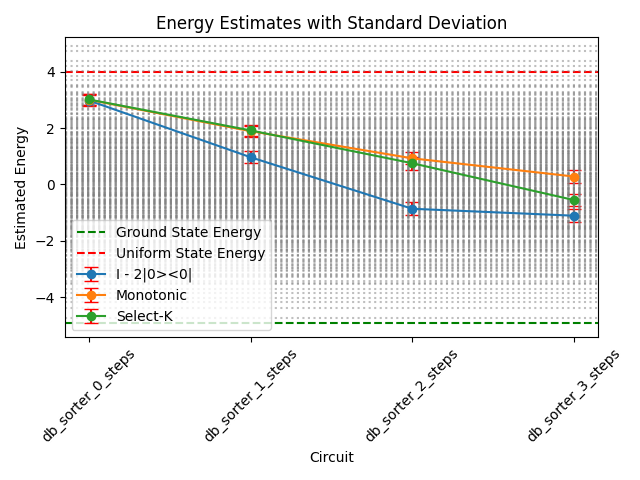
\includegraphics[width=\textwidth]{TFIM_diagonals.png}
        \caption{TFIM model}
        \label{subfig:tfim-diag}
    \end{subfigure}
    \hfill
    \begin{subfigure}[b]{0.45\textwidth}
        \centering
        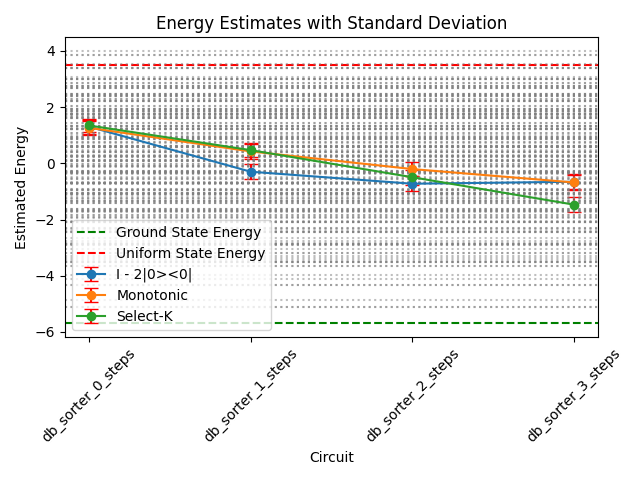
\includegraphics[width=\textwidth]{XXZ_diagonals.png}
        \caption{XXZ model}
        \label{subfig:xxz-diag}
    \end{subfigure}
    
    \vspace{0.5cm} % Adds vertical spacing between the rows
    
    % === SECOND ROW ===
    \begin{subfigure}[b]{0.45\textwidth}
        \centering
        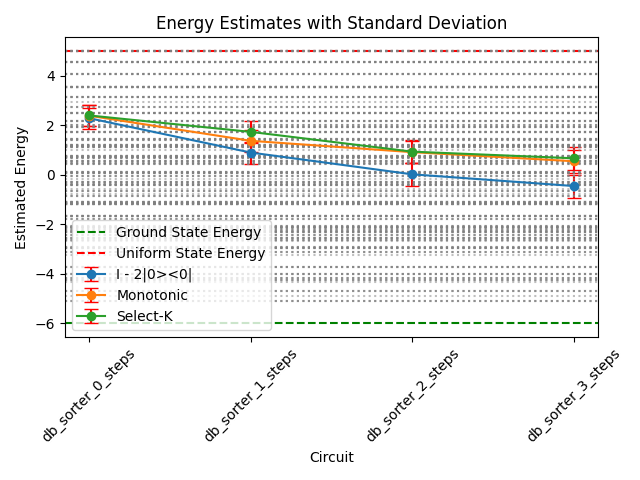
\includegraphics[width=\textwidth]{J1_J2_diagonals.png}
        \caption{J1/J2 model}
        \label{subfig:j1-j2-diag}
    \end{subfigure}
    % \hfill
    % \begin{subfigure}[b]{0.45\textwidth}
    %     \centering
    %     \includegraphics[width=\textwidth]{monotone_4_steps.png}
    %     \caption{Modified Grover is more resistance to divergence.}
    %     \label{subfig:monotone-4}
    % \end{subfigure}

    % === MAIN CAPTION ===
    \caption{All models show a cool down behaviour. Projection consistently starts sharper and faster and for most cases select-k, as expected, ends up second. We had similar pattern for $H_2$ and $NH_3$}
    \label{fig:model-comparison}
\end{figure}



\subsubsection{Scaling with the number of qubits}
\label{sec:scaling}
Scaling (and fidelity in general) did not prove to be promising with cold-start. You can see the results in \hyperref[fig:model-scaling]{Figure 2}

\begin{figure}[htbp]
    \centering
    % === FIRST ROW ===
    \begin{subfigure}[b]{0.9\textwidth}
        \centering
        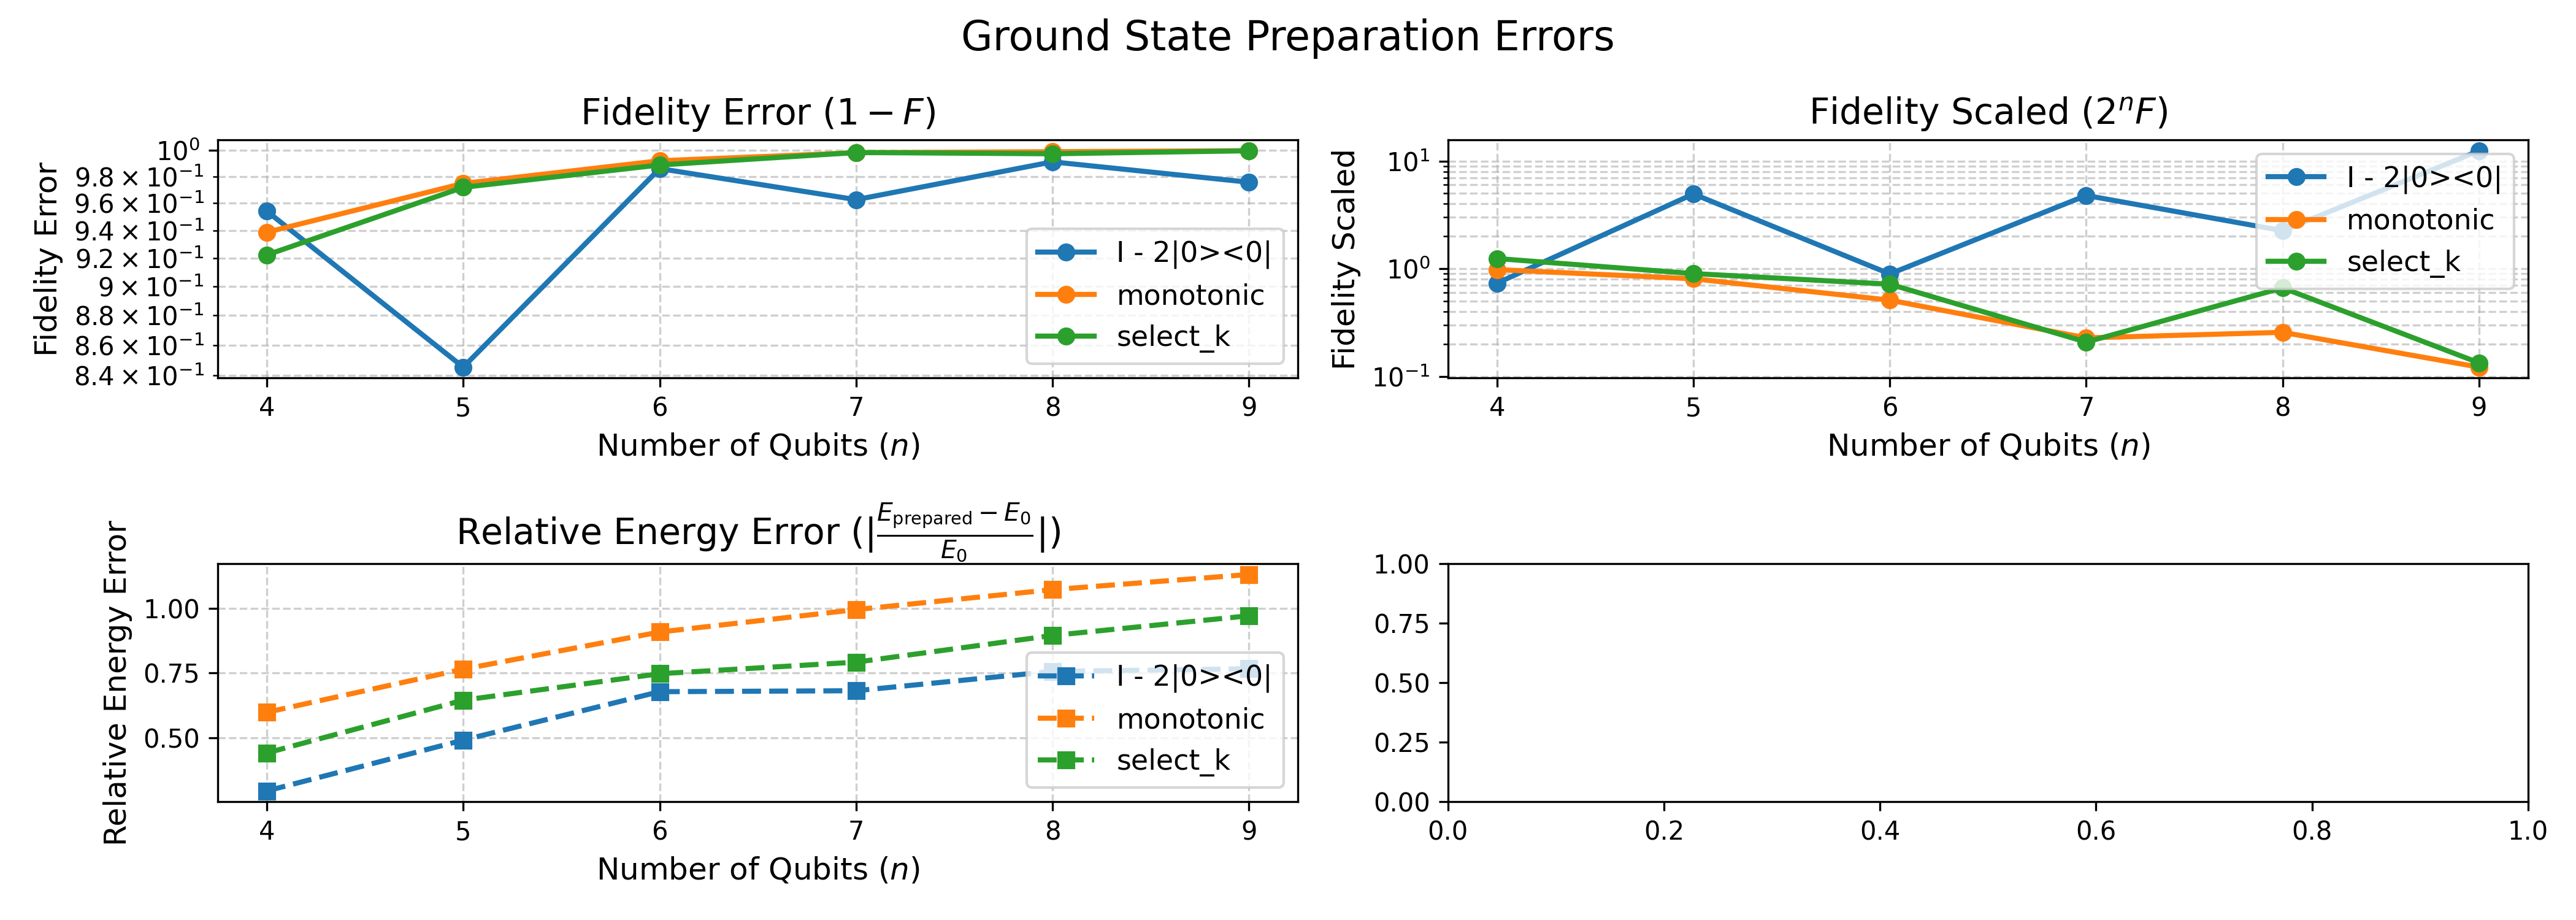
\includegraphics[width=\textwidth]{TFIM_scaling.png}
        \caption{TFIM model}
        \label{subfig:tfim-diag}
    \end{subfigure}

    \vspace{0.5cm} % Adds vertical spacing between the rows
    
    \begin{subfigure}[b]{0.9\textwidth}
        \centering
        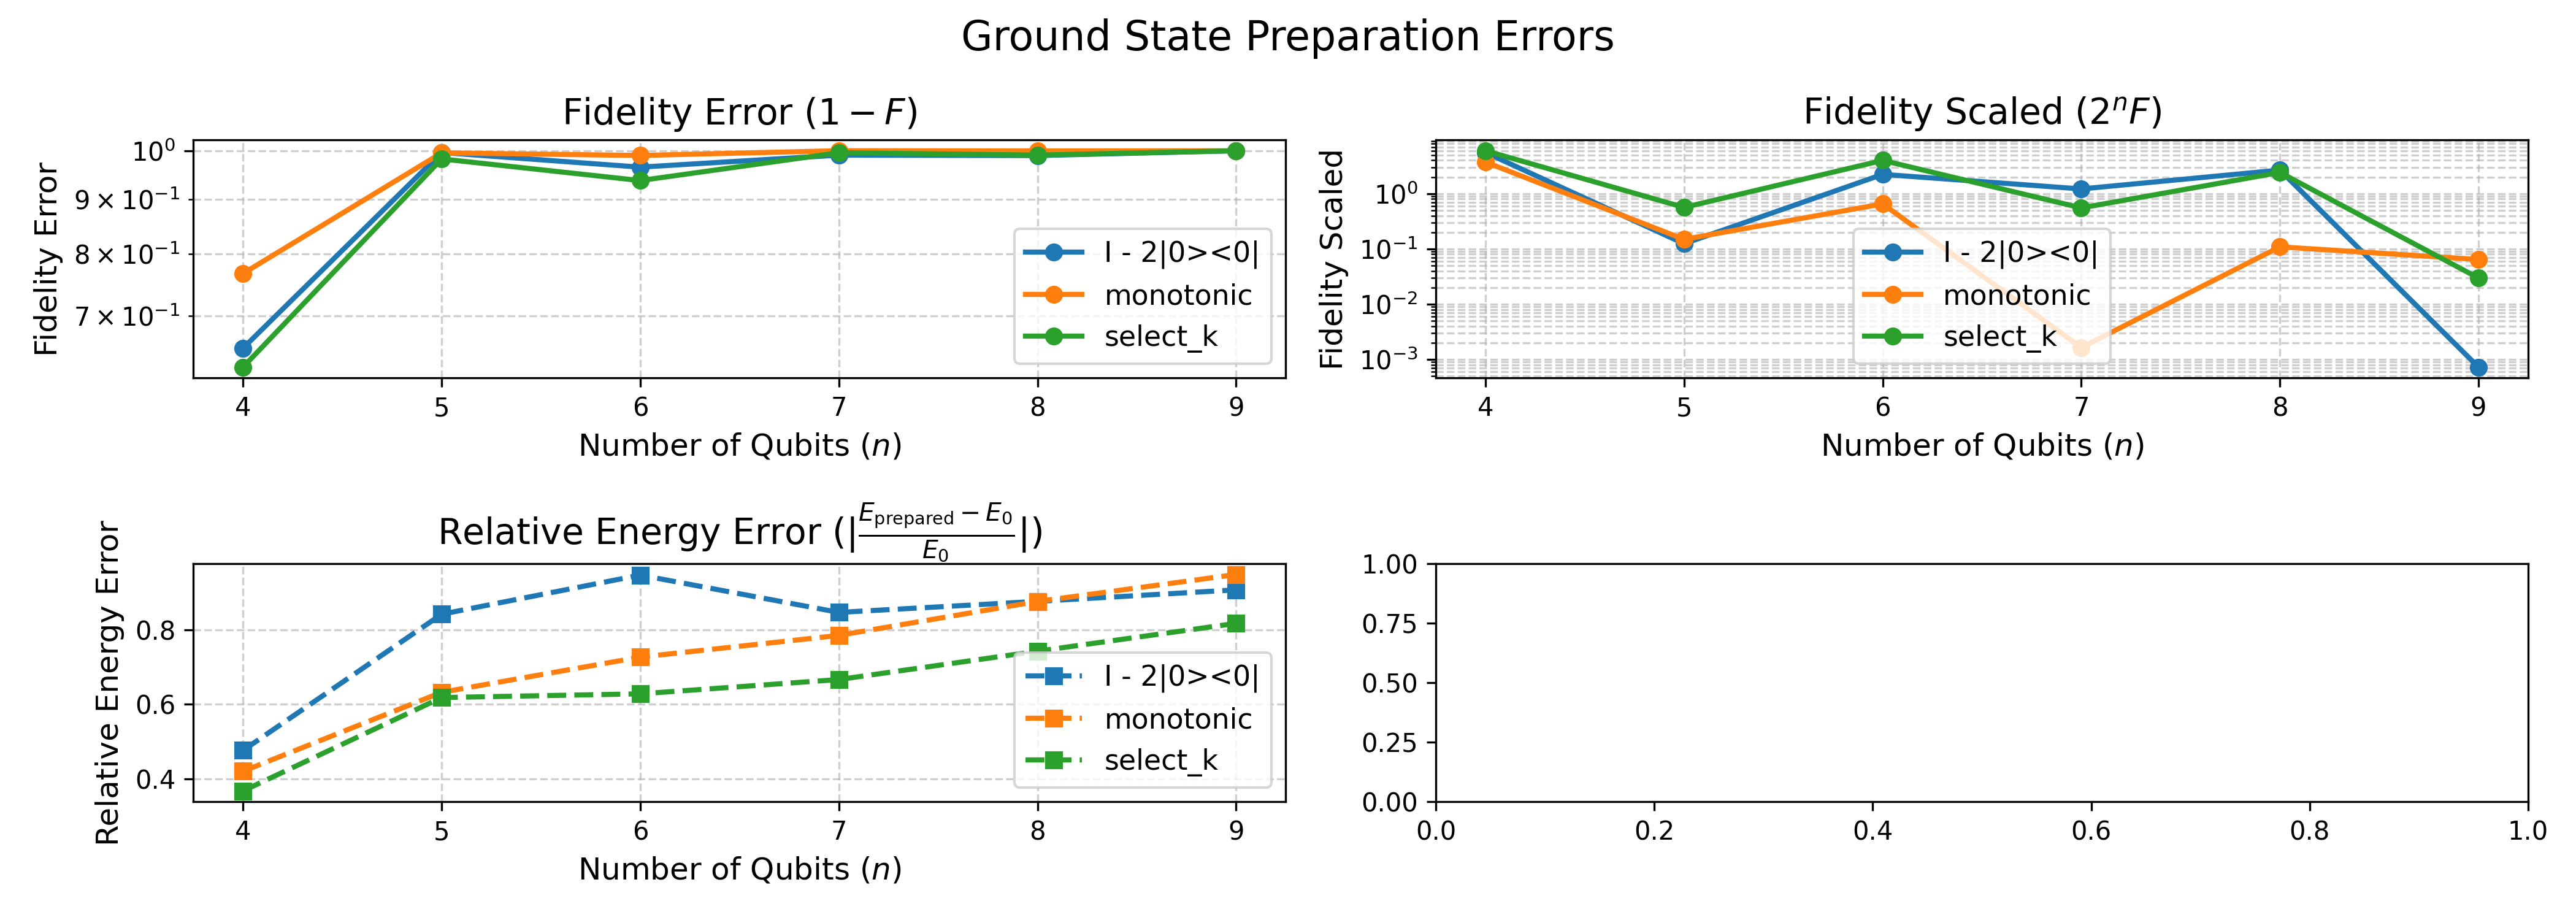
\includegraphics[width=\textwidth]{XXZ_scaling.png}
        \caption{XXZ model}
        \label{subfig:xxz-diag}
    \end{subfigure}
    
    \vspace{0.5cm} % Adds vertical spacing between the rows
    
    % === SECOND ROW ===
    \begin{subfigure}[b]{0.9\textwidth}
        \centering
        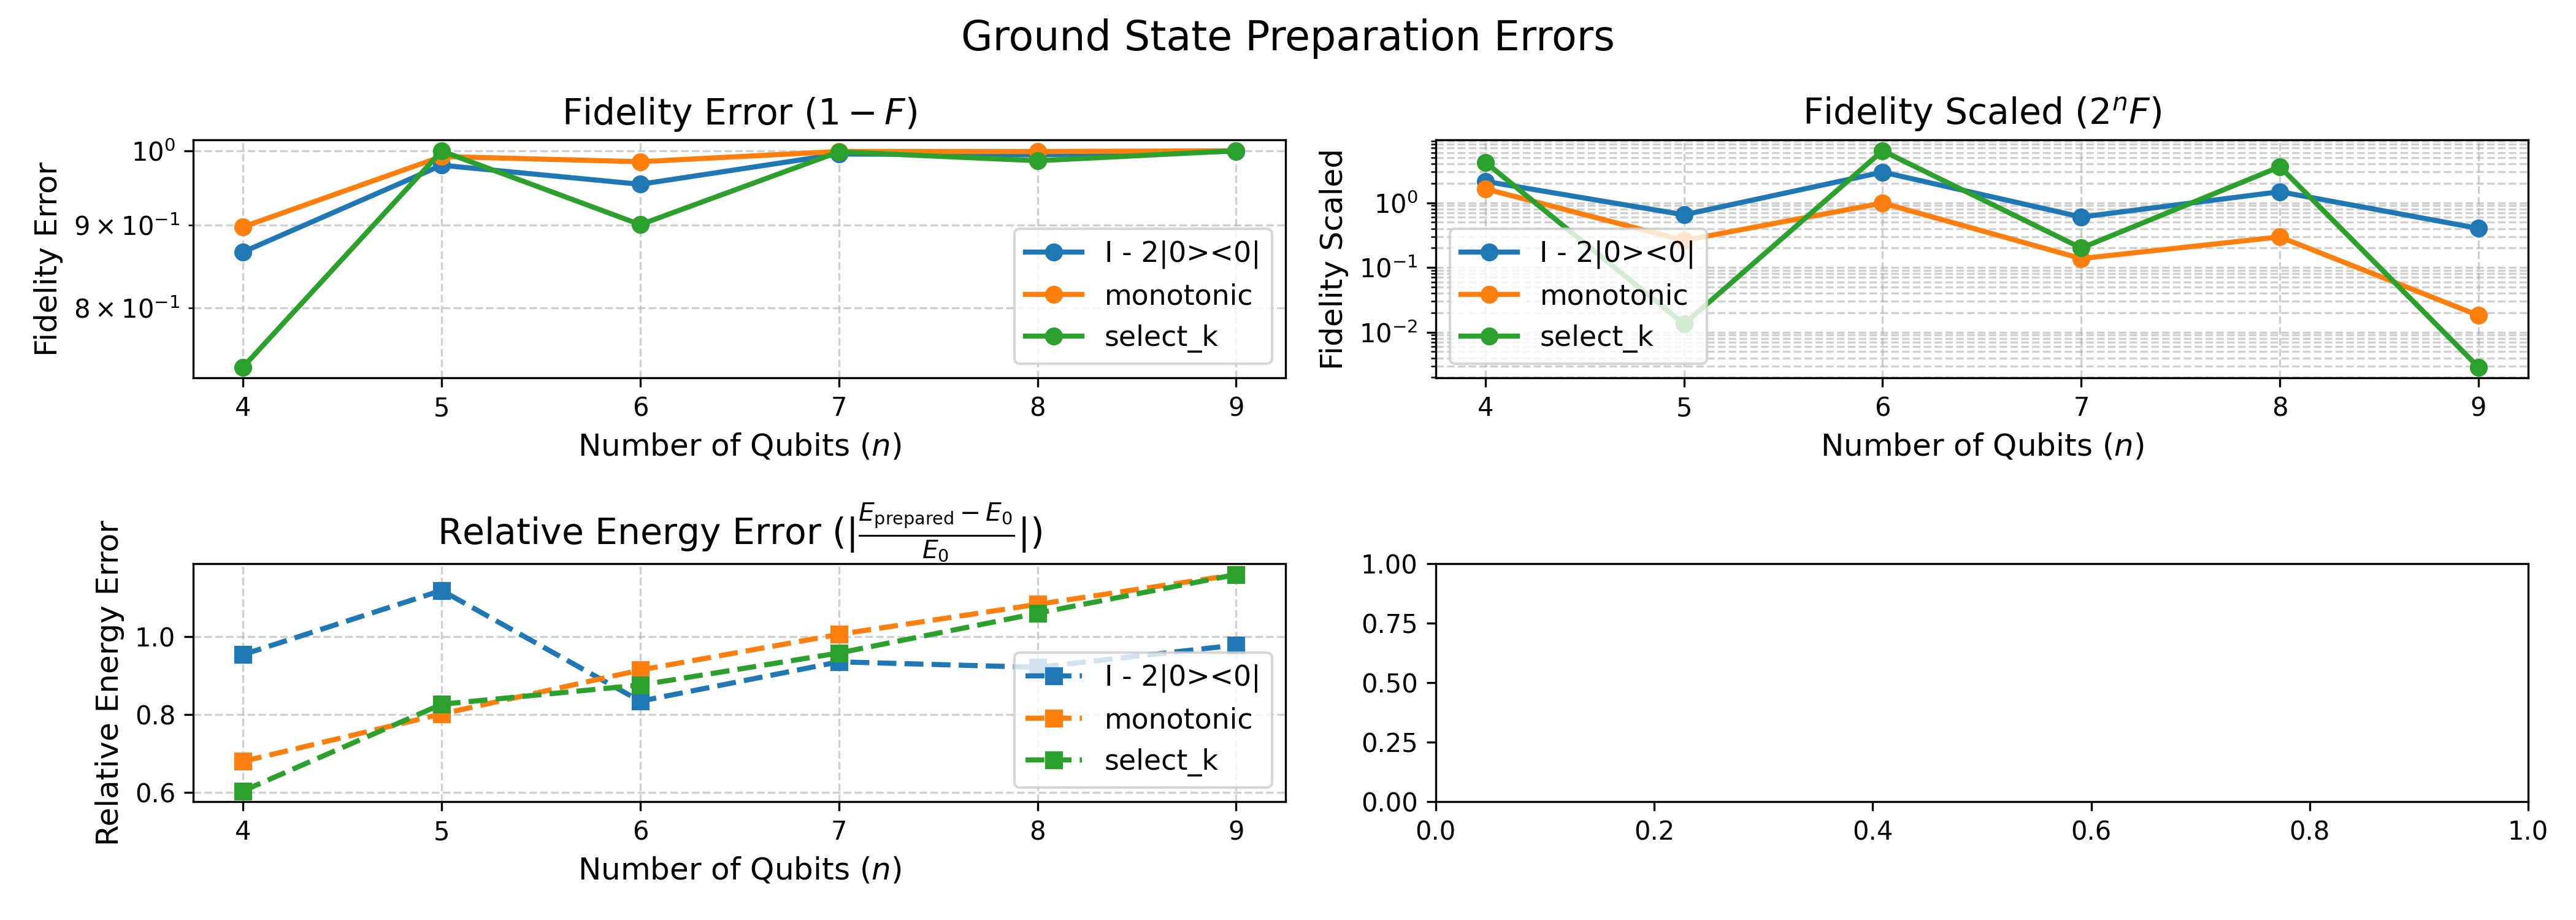
\includegraphics[width=\textwidth]{J1_J2_scaling.png}
        \caption{J1/J2 model}
        \label{subfig:j1-j2-diag}
    \end{subfigure}
    % \hfill
    % \begin{subfigure}[b]{0.45\textwidth}
    %     \centering
    %     \includegraphics[width=\textwidth]{monotone_4_steps.png}
    %     \caption{Modified Grover is more resistance to divergence.}
    %     \label{subfig:monotone-4}
    % \end{subfigure}

    % === MAIN CAPTION ===
    \caption{The fidelity is not promising with cold-start}
    \label{fig:scaling}
\end{figure}

\end{document}
